
%(BEGIN_QUESTION)
% Copyright 2007, Tony R. Kuphaldt, released under the Creative Commons Attribution License (v 1.0)
% This means you may do almost anything with this work of mine, so long as you give me proper credit

Sometimes two or more separate control loops interact with one another by way of the process being controlled.  When this happens, the loops are said to be {\it coupled}.  An example of this is air flow and air pressure control on a large combustion furnace:

$$\includegraphics[width=15.5cm]{i01771x01.eps}$$

The flow controller (FC) works to maintain a set air flow into the furnace for combustion, in order to precisely control the firing rate of the burner.  The pressure controller (PC) works to maintain a constant furnace box pressure, to ensure minimal leakage of cold air into the furnace, or hot air out of the furnace.

\vskip 10pt

A simple ``thought experiment'' illustrates the problem of coupling: suppose the setpoint to the flow controller is suddenly increased, calling for more air (to fuel a larger fire).  What happens to furnace pressure as the inlet air flow damper opens up?  What does the pressure controller tell the exhaust stack damper to do in order to maintain constant furnace pressure?  How does the stack damper's motion consequently affect the air flow into the furnace?  Unless one of these controllers is tuned much faster than the other, the two control systems will tend to ``fight'' one another through coupling.

\vskip 10pt

\filbreak

A solution to this control problem is {\it decoupling}, illustrated in the next diagram:

$$\includegraphics[width=15.5cm]{i01771x02.eps}$$

Explain how this control system modification solves the problem of coupling, and also explain how it is similar to {\it feedforward control} in its design.

\underbar{file i01771}
%(END_QUESTION)





%(BEGIN_ANSWER)

Since the stack damper is actuated by the flow controller's output in addition to the pressure controller's output, it will move in tandem with the inlet air damper to minimize the effect on furnace pressure.  The pressure controller then merely serves a ``trim'' function.

\vskip 10pt

Challenge question: true feedforward control would look something like this, but it would {\it not} fix the coupling problem.  Explain why:

$$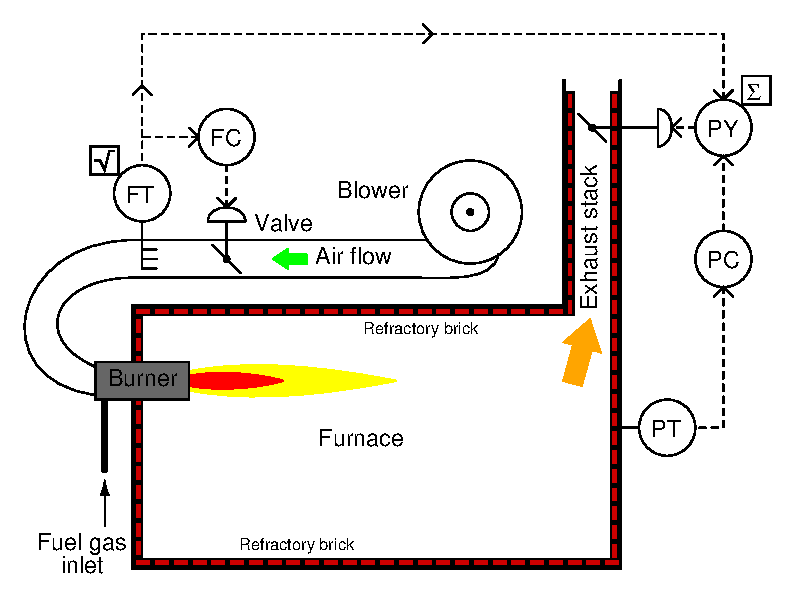
\includegraphics[width=15.5cm]{i01771x03.eps}$$

%(END_ANSWER)





%(BEGIN_NOTES)

In the challenge question, the feedforward signal sent to the stack damper actually constitutes a {\it positive feedback} signal for the flow controller, inviting instability.

%INDEX% Control, strategies: decoupling
%INDEX% Control, strategies: feedforward
%INDEX% Process: combustion furnace

%(END_NOTES)


